% !TEX root = ../main.tex

\section{Methodology}
\label{sec:methodology}

The first experimental part of the project answers a profiling question: \emph{where does the time of one SmolVLA~\cite{smolvla2025} inference go on an NPU, and how does the split change when the NPU becomes an edge-class device?} We use PyTorchSim~\cite{pytorchsim} as an end-to-end, cycle-level simulator of the whole model, and SCALE-Sim~v3~\cite{samajdar2020scalesim,scalesimv3} only as a cross-check of single GEMMs; the GEMM-level design-space exploration with SCALE-Sim is the next part of the project. All code, configurations and summary data are in the project repository (\texttt{src/p1\_profiling/}, \texttt{configs/pytorchsim/}, \texttt{results/}).

\subsection{The SmolVLA workload}
\label{subsec:method-workload}

One inference of SmolVLA (\texttt{smolvla\_base}, 3 cameras) produces an \emph{action chunk} of $H=50$ actions. We split it into four stages (\cref{fig:smolvla-workload,tab:stages}): the SigLIP vision encoder, run once per camera; the connector (pixel-shuffle and projection to the VLM width); the \emph{prefix}, i.e.\ the 16-layer SmolVLM2 backbone over the $3\times 64$ image tokens, 48 language tokens and the state token (241 tokens), which produces the KV cache; and one flow-matching \emph{denoise} step of the action expert over the 50 action tokens, repeated 10 times ($\delta = 0.1$). The prefix KV cache is computed once and reused by all denoise steps, so the stages are strictly sequential within a chunk:
\begin{equation}
  T_\text{chunk} = 3\,(T_\text{vision} + T_\text{connector}) + T_\text{prefix} + 10\,T_\text{denoise}.
  \label{eq:chunk}
\end{equation}

\begin{table}[tp]
\centering
\small
\caption{SmolVLA stages (fp32, batch 1), per instance; \emph{runs} is the number of instances per action chunk. FLOPs from the exact GEMM trace of \texttt{sample\_actions}; compulsory traffic and arithmetic intensity as in \cref{subsec:method-roofline}; activation is one token-by-width tensor (in brackets: the MLP hidden one).}
\label{tab:stages}
\setlength{\tabcolsep}{4pt}
\begin{tabular}{l c r r r r r r r}
\toprule
Stage & Runs & Tokens & Width & Layers & GFLOP & Compulsory MB & FLOP/B & Activation MB \\
\midrule
Vision encoder & 3 & 1024 & 768 & 12 & 213.8 & 349 & 613 & 3.1 (12.6) \\
Connector & 3 & 64 & $12288{\to}960$ & 1 & 1.5 & 51 & 30 & 3.1 \\
Prefix (VLM) & 1 & 241 & 960 & 16 & 79.4 & 641 & 124 & 0.9 (2.5) \\
Denoise step & 10 & 50 & 720 & 16 & 11.3 & 410 & 28 & 0.14 (0.41) \\
\bottomrule
\end{tabular}
\end{table}

\begin{figure}[tp]
\centering
\resizebox{\textwidth}{!}{% !TEX root = ../main.tex
% SmolVLA as a workload: block height is proportional to the number of tokens of each stage.
\begin{tikzpicture}[
    font=\footnotesize,
    blk/.style={draw=#1, fill=#1!18, line width=0.8pt},
    lab/.style={align=center, inner sep=1pt},
    arr/.style={-{Stealth[length=2mm]}, line width=0.7pt, draw=black!70},
  ]
  \def\h{3.2/1024}   % cm per token
  % ---- input: one camera image at a time (3 cameras -> vision and connector run 3 times)
  \draw[fill=black!8, draw=black!50] (0, 1.15) rectangle ++(0.9, 0.9);
  \node[lab, above] at (0.45, 2.1) {1 camera\\$512{\times}512$};
  % ---- vision encoder: 1024 tokens
  \draw[blk=visc] (1.9, 0) rectangle (4.5, 3.2);
  \node[lab] at (3.2, 1.6) {\textbf{Vision encoder}\\(SigLIP)\\[2pt]12 layers\\$d{=}768$, MLP 3072\\[2pt]\textbf{1024 tokens}};
  \draw[visc!80!black, line width=0.7pt] (0, 3.35) -- (0, 3.5) -- node[lab, above] {\textbf{$\times$3} cameras, one image at a time} (6.9, 3.5) -- (6.9, 3.35);
  \draw[arr] (0.95, 1.6) -- node[lab, above] {\scriptsize $16{\times}16$} node[lab, below] {\scriptsize patches} (1.85, 1.6);
  % ---- connector: 64 tokens per camera
  \draw[blk=conc] (5.4, 0) rectangle (6.9, 64*\h);
  \node[lab, above] at (6.15, 64*\h) {\textbf{Connector}\\pixel shuffle\\+ linear\\\textbf{64 tokens}};
  \draw[arr] (4.5, 0.1) -- (5.4, 0.1);
  % ---- prefix: 192 image + 48 text + 1 state = 241 tokens
  \draw[blk=prec] (8.1, 0) rectangle (10.7, 241*\h);
  \node[lab, above] at (9.4, 241*\h) {\textbf{VLM prefix} (SmolVLM2)\\16 layers, $d{=}960$, MLP 2560\\[2pt]\textbf{241 tokens} = 192 image\\+ 48 text + 1 state};
  \draw[arr] (6.9, 0.1) -- node[lab, below=1pt] {\scriptsize $3{\times}64$} (8.1, 0.1);
  \node[lab, anchor=north] (txt) at (9.4, -0.55) {task text, robot state};
  \draw[arr] (txt.north) -- (9.4, 0);
  % ---- action expert: 50 tokens, 10 steps
  \draw[blk=denc] (12.4, 0) rectangle (15.0, 50*\h);
  \node[lab, above] at (13.7, 50*\h+0.95) {\textbf{Action expert}\\16 layers, $d{=}720$, MLP 2048\\[2pt]\textbf{50 tokens} (the action chunk)};
  \draw[arr] (10.7, 0.1) -- node[lab, above] {\scriptsize KV cache} node[lab, below=1pt] {\scriptsize 241 keys} (12.4, 0.1);
  \draw[arr, draw=denc!80!black] (15.0, 0.08) -- ++(0.35, 0) -- ++(0, 0.45) -- node[lab, above] {\textbf{$\times$10} denoise steps} ++(-2.95, 0) -- ++(0, -0.3);
  \node[lab, anchor=north] (noise) at (13.7, -0.55) {noisy actions};
  \draw[arr] (noise.north) -- (13.7, 0);
  \draw[arr] (15.35, 0.08) -- (16.0, 0.08) node[lab, right] {50\\actions};
  % ---- arithmetic intensity row
  \draw[black!30] (-0.1, -1.15) -- (16.9, -1.15);
  \node[lab, anchor=west] at (-0.1, -1.5) {FLOP/B (fp32):};
  \node[lab] at (3.2, -1.5) {\textbf{613}};
  \node[lab] at (6.15, -1.5) {\textbf{30}};
  \node[lab] at (9.4, -1.5) {\textbf{124}};
  \node[lab] at (13.7, -1.5) {\textbf{28}};
\end{tikzpicture}
}
\caption{SmolVLA as a workload. Every stage is a stack of transformer layers; what differs is the number of tokens that flows through them (block height, to scale) and how often the stage runs per action chunk. The bottom row is the arithmetic intensity with compulsory traffic (\cref{tab:stages}).}
\label{fig:smolvla-workload}
\end{figure}

\paragraph{Tokens set the regime.} All four stages are transformers, so what separates them is the number of tokens $M$ each weight is applied to. A linear layer of $K{\times}N$ weights does $2MNK$ FLOPs while reading $4NK$ bytes of fp32 weights, so its arithmetic intensity is about $M/2$~FLOP/B, linear in the tokens: about 500 for vision ($M=1024$), 120 for the prefix ($M=241$) and 25 for the action expert ($M=50$), close to the values of \cref{tab:stages}. The quadratic attention term ($4M^2d$ FLOPs per layer) adds about a fifth to vision's FLOPs and is negligible in the other stages. Against the ridge points of the simulated NPUs (40--640~FLOP/B, \cref{tab:npus}), vision is therefore compute-bound and the action expert memory-bound: it streams its ${\approx}400$~MB of weights for only 50 tokens, in each of the 10 steps.

\paragraph{Static re-implementation.} The lerobot implementation cannot be compiled as a whole (dynamic masks, image resizing, cache objects and a Python denoising loop). We therefore re-implemented each layer type and each stage as static-shape PyTorch modules that load the real checkpoint weights. A CPU check against lerobot's own code passes for every stage with a relative error below $10^{-5}$. Independently, a \texttt{TorchDispatchMode} hook on lerobot's real \texttt{sample\_actions} records every GEMM with its exact $(M,N,K)$ and phase: 1919 GEMMs and 839.6~GFLOP per chunk, 28 unique shapes; the per-stage FLOPs match those of the re-implementation exactly.

\subsection{PyTorchSim}
\label{subsec:method-pytorchsim}

PyTorchSim~\cite{pytorchsim} has two parts (\cref{fig:pytorchsim-overview}): a compiler that turns a PyTorch model into NPU code, and TOGSim, which simulates that code on a configurable NPU.

\begin{figure}[tp]
\centering
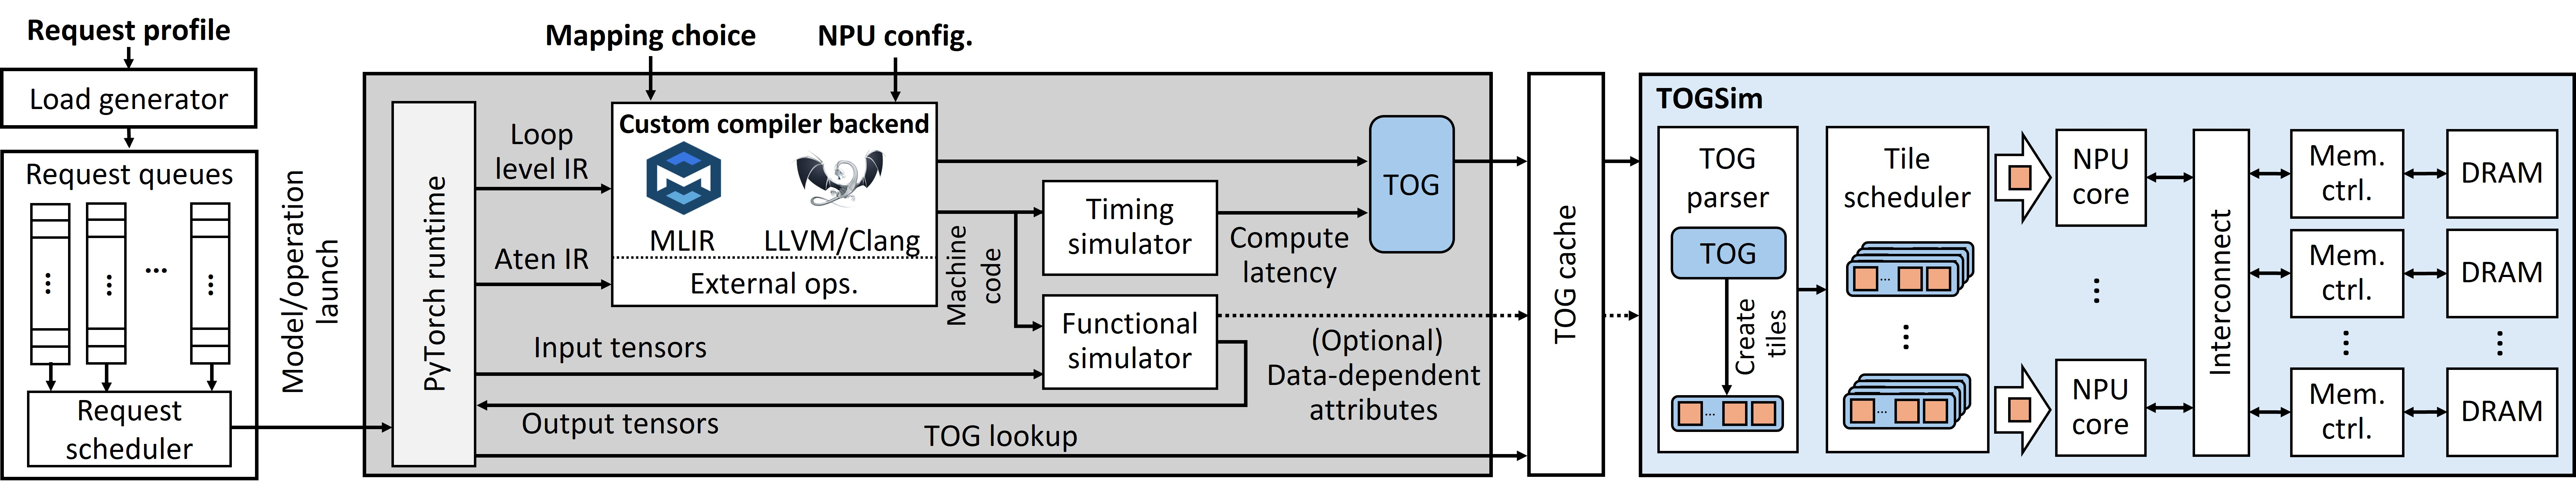
\includegraphics[width=\textwidth]{6.1-pytorchsim-overview.jpg}
\caption{PyTorchSim overview, credits \cite{pytorchsim}. The compiler backend lowers each kernel to machine code and to a tile-operation graph (TOG); TOGSim replays the TOGs on NPU cores, an interconnect and DRAM.}
\label{fig:pytorchsim-overview}
\end{figure}

\paragraph{Compiler.} A model is compiled with \texttt{torch.compile} for a PyTorch device, \texttt{npu:0}, that stands for the simulated NPU. Inductor splits the model into fused kernels and lowers each one either to an MLIR template (GEMM, convolution, a fused flash-attention template~\cite{dao2022flashattention}) or to generated vector code, and then to a RISC-V binary. The \emph{mapping} step chooses the tile sizes of each kernel, by default with a heuristic adopted from Gemmini that maximises the use of the scratchpad. Each kernel becomes a \emph{tile-operation graph} (TOG): the sequence of tile loads (DMA), matrix and vector operations and stores, with their dependencies. The latency of each compute node of the TOG is measured once by running its code on a timing simulator (gem5); an optional functional mode runs the binary on Spike to check the output values.

\paragraph{TOGSim.} TOGSim parses the TOGs, creates the tiles and schedules them on the NPU cores. It models the cores at the level of tile operations, and the shared resources cycle by cycle: the interconnect (a simple latency model in our configurations, optionally BookSim) and the memory controllers and DRAM (Ramulator~2~\cite{luo2023ramulator2}). Because the compute latencies come from the TOG, a whole model is simulated much faster than with a cycle-level model of the core, while DRAM contention and bandwidth stay accurate. A core (\cref{fig:pytorchsim-core}) has a scalar unit and control, $\ell$ vector lanes, each with its functional units, register file and slice of the scratchpad, a DMA engine to DRAM, and one or more dataflow units (weight-stationary systolic arrays) fed from the vector registers. In PyTorchSim the systolic array is $\ell \times \ell$, so the array, the vector width and the (per-lane) scratchpad scale together.

\begin{figure}[tp]
\centering
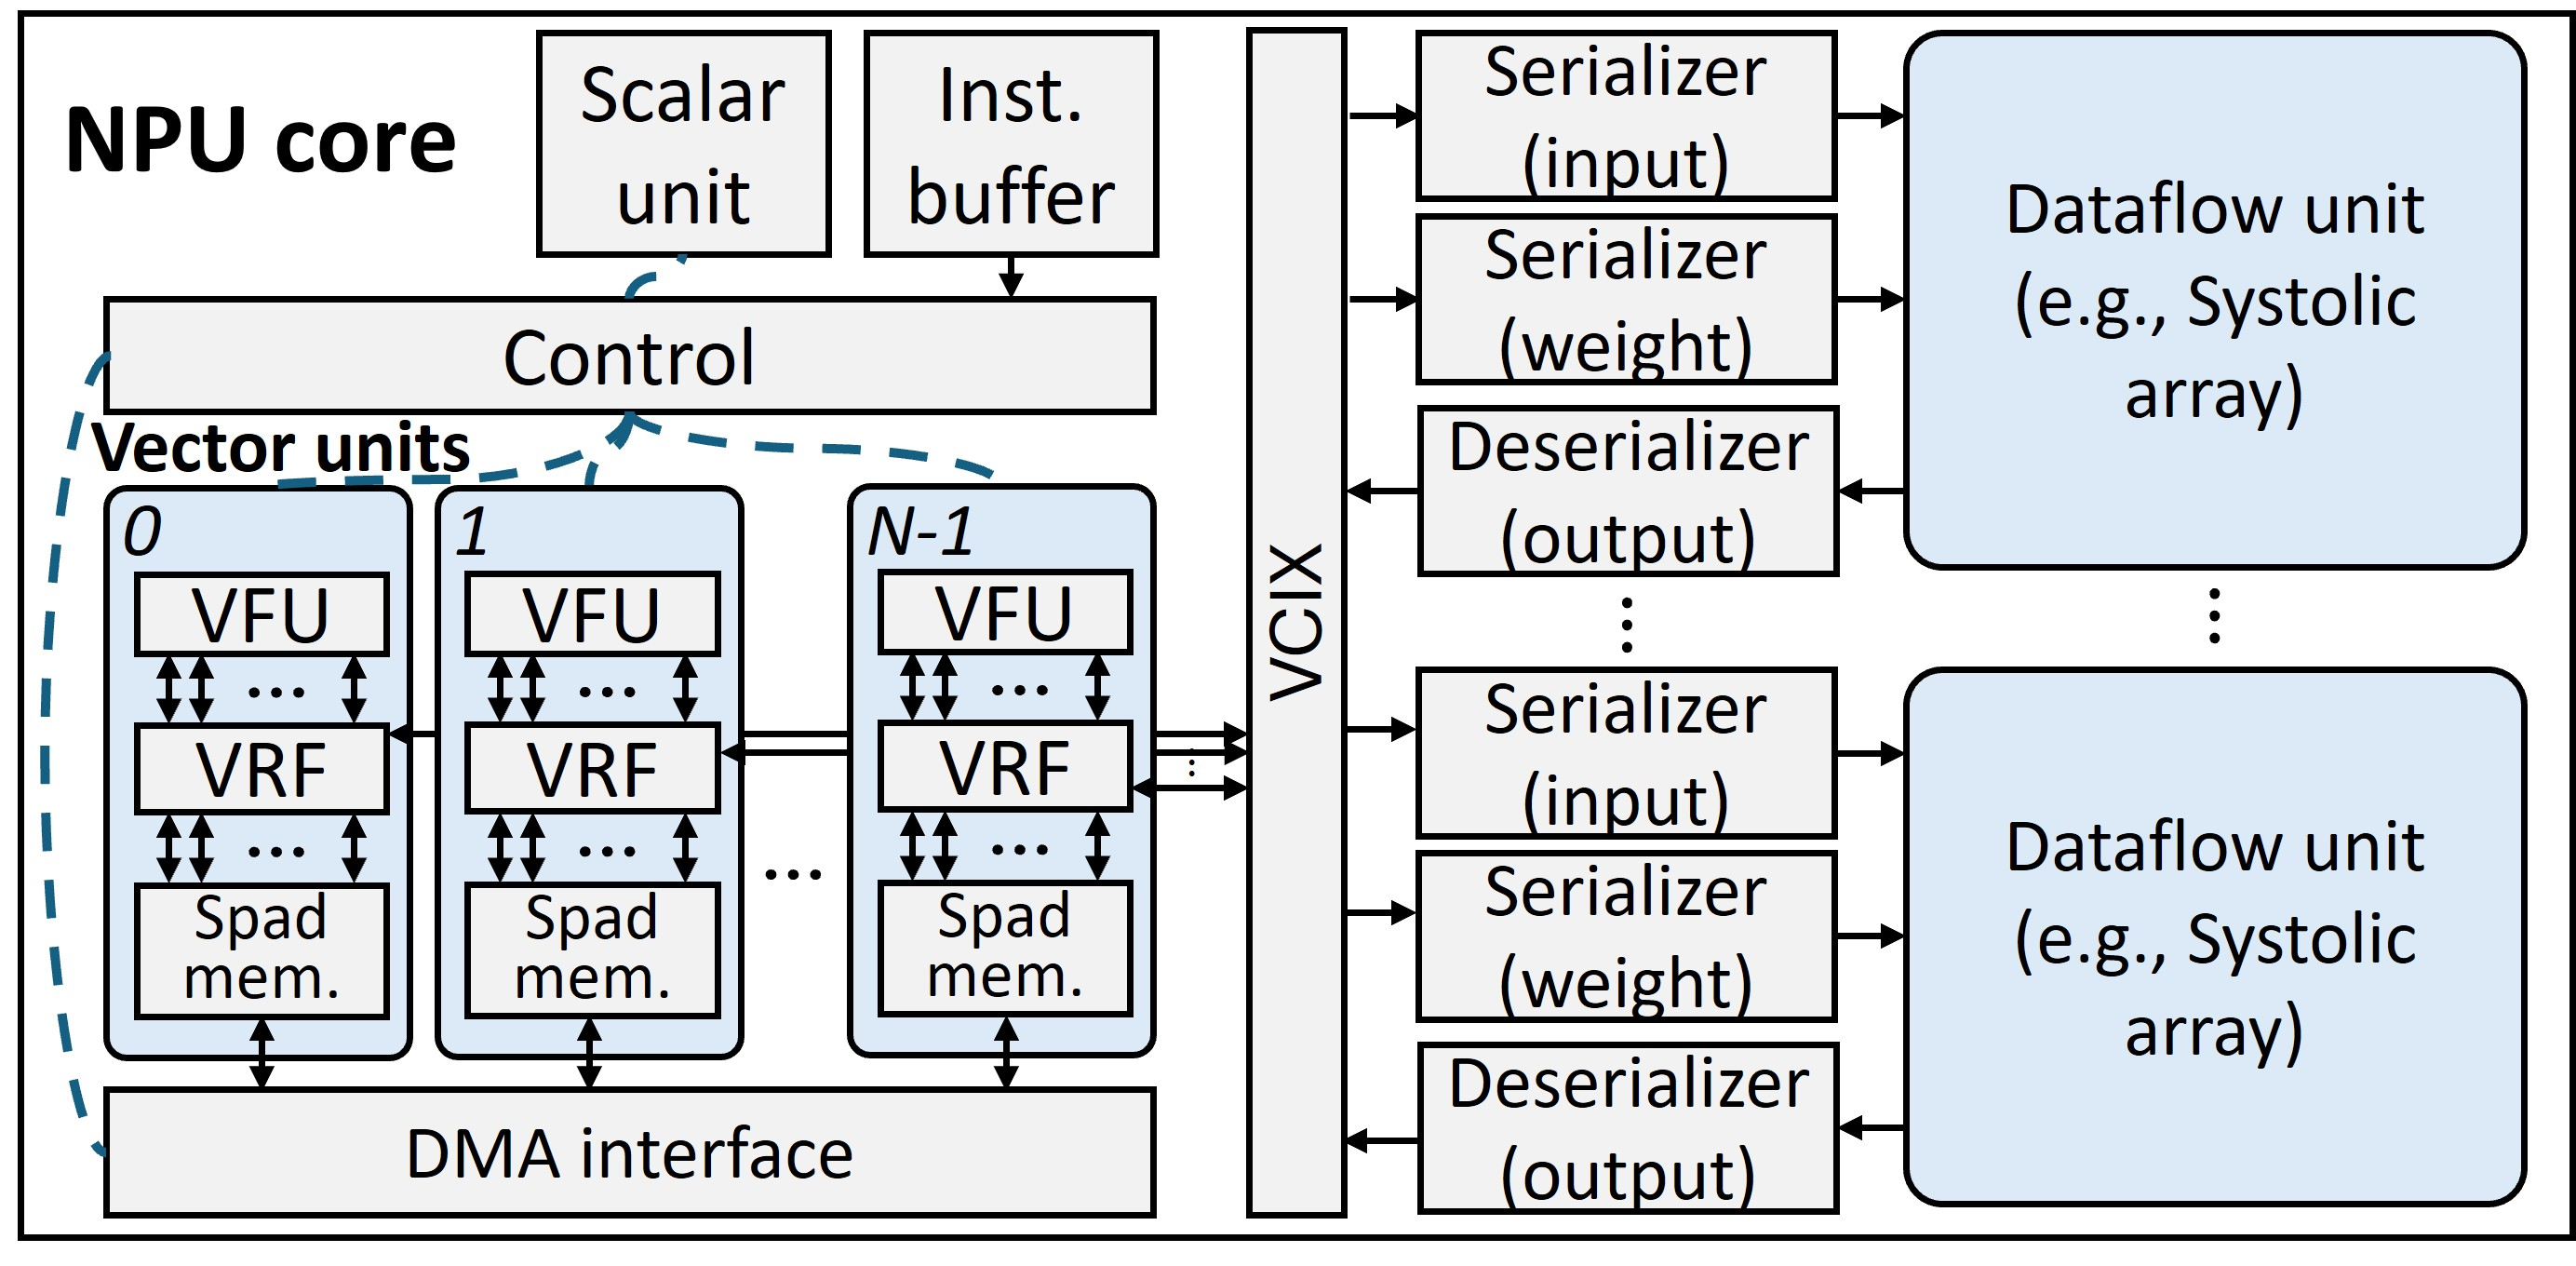
\includegraphics[width=0.6\textwidth]{6.2-pytorchsim-npu-core.jpg}
\caption{NPU core modelled by TOGSim, credits \cite{pytorchsim}: vector lanes with scratchpad (Spad), DMA interface, and systolic arrays fed through serializers.}
\label{fig:pytorchsim-core}
\end{figure}

We run each stage, or the full chunk, as a sequence of launches in a single TOGSim session, with a synchronisation after each launch (the stage dependency). Each kernel's start cycle and duration are attributed to its stage, which gives the per-stage time inside the one-session chunk run and a breakdown by kernel type. Three choices in how the model is fed to the compiler turned out to change the results more than the effects under study:
\begin{dashlist}
  \item the $16{\times}16$, stride-16 patch convolution is rewritten as a host-side reshape plus a $1024{\times}768{\times}768$ GEMM (the convolution template used $3$ of $128$ array rows: $7.2\times$ faster);
  \item the vision attention uses PyTorchSim's fused flash template ($-43\%$ DRAM traffic per layer); the VLM and expert attentions cannot (grouped-query heads, masks, $L \neq S$) and run as matmul plus softmax;
  \item all runs use PyTorchSim's \emph{heuristic} tile mapping: the autotuner selects kernels that TOGSim then times at 0--1 cycles inside a session, which inflates its apparent speed-up.
\end{dashlist}
All simulations are fp32 at batch 1: the 16-bit paths of the toolchain fail on layers with normalisations. Timing is data-independent for these dense kernels, so random inputs are used in the timing runs.

\subsection{Simulated NPUs}
\label{subsec:method-npus}

\Cref{tab:npus} lists the configurations. The \emph{big} NPU is a TPUv3-like reference shipped with PyTorchSim. The edge candidates use one $\ell\times\ell$ array at 1~GHz with LPDDR5-6400 (12.8~GB/s per x16 channel). The sweeps vary the DRAM bandwidth at a fixed $64\times64$ array, and the array size at a fixed 51.2~GB/s.

\begin{table}[tp]
\centering
\small
\caption{Simulated NPU configurations (fp32 peak; ridge point = peak FLOP/s over DRAM bandwidth).}
\label{tab:npus}
\setlength{\tabcolsep}{4pt}
\resizebox{\textwidth}{!}{%
\begin{tabular}{l l r r r r}
\toprule
Configuration & Arrays & Peak (TFLOP/s) & Scratchpad & DRAM (GB/s) & Ridge (FLOP/B) \\
\midrule
Big (TPUv3-like) & $2 \times 128{\times}128$, 940~MHz & 61.6 & 16~MB & HBM2, 481 & 128 \\
Edge $64{\times}64$ & $1 \times 64{\times}64$ & 8.2 & 4~MB & LPDDR5 $\times4$, 51.2 & 160 \\
Edge $32{\times}32$ & $1 \times 32{\times}32$ & 2.0 & 2~MB & LPDDR5 $\times4$, 51.2 & 40 \\
Bandwidth sweep & $1 \times 64{\times}64$ & 8.2 & 4~MB & LPDDR5 $\times1$--$\times16$, 12.8--205 & 640--40 \\
Array sweep & $1 \times \{32,128\}^2$ & 2.0 / 32.8 & 4~MB & LPDDR5 $\times4$, 51.2 & 40 / 640 \\
\bottomrule
\end{tabular}}
\end{table}

\subsection{Roofline reference}
\label{subsec:method-roofline}

To separate what the hardware could do from what PyTorchSim's compiler achieves, every stage is compared with a roofline model~\cite{10.1145/1498765.1498785}. With $F$ the GEMM FLOPs (from \texttt{FlopCounterMode}) and $Q$ the \emph{compulsory} DRAM traffic (weights, inputs and outputs, each moved once), the ideal time of a stage on an NPU with peak $P$ and bandwidth $B$ is
\begin{equation}
  T_\text{ideal} = \max\!\left(\frac{F}{P},\ \frac{Q}{B}\right),
  \label{eq:ideal}
\end{equation}
i.e.\ the time of a perfectly tiled NPU with the same array and DRAM. Substituting $T_\text{ideal}$ in \cref{eq:chunk} gives the \emph{ideal} stage shares, reported next to the simulated ones. The measured DRAM traffic comes from Ramulator's request counts; its ratio to $Q$ quantifies the extra traffic of the generated tiling.

\subsection{Time and traffic attribution}
\label{subsec:method-attribution}

Totals and roofline bounds do not say \emph{why} a stage is slow. TOGSim saves the launch list of each run and can replay it standalone, cycle for cycle, from the compiled tile graphs; at its most verbose log level it reports every instruction with its issue and finish cycle, its unit (systolic array or vector unit), and, for DMA instructions, the tensor, address and tile shape. We replay every stage run this way (the replay reproduces the original cycle count, and its DMA requests match the DRAM model's counts exactly) and derive two breakdowns:
\begin{dashlist}
  \item \textbf{time}: each cycle is \emph{array busy} (a matrix instruction in flight), \emph{vector unit only}, \emph{waiting on DRAM only}, or \emph{other}; the array-busy time is further split into \emph{streaming} (TOGSim's own active-cycle count) and unhidden pipeline fill/drain;
  \item \textbf{traffic}: each DRAM line moved is \emph{compulsory} (first read of weights and inputs, outputs written once), a \emph{kernel-boundary round trip} (an activation written by one kernel and read back by a later one, which fusion would keep on chip), a \emph{weight re-read} (a weight or input line read again, by the tiling or by a later kernel), or an \emph{activation re-read} (an activation read again inside the same kernel, which only a different tiling or a larger scratchpad removes).
\end{dashlist}

To separate the compiler from the hardware, we also re-simulate with \emph{forced tiling}: PyTorchSim's heuristic picks the GEMM tile that fills the most scratchpad, so we enumerate the same feasible tiles and select, for each of the GEMM shapes, the one with the least modelled DRAM traffic, which PyTorchSim then uses through its external mapping interface. Functional checks against the CPU reference give the same errors as with the heuristic tiles.

\subsection{SCALE-Sim cross-check}
\label{subsec:method-scalesim}

Six representative GEMMs (vision, VLM and expert shapes) were run on one $64\times64$ weight-stationary array in both simulators, compute-bound on both sides (PyTorchSim with HBM2, SCALE-Sim~v3 with a stall-free interface), and compared with the ideal $MNK/64^2$ cycles.
